	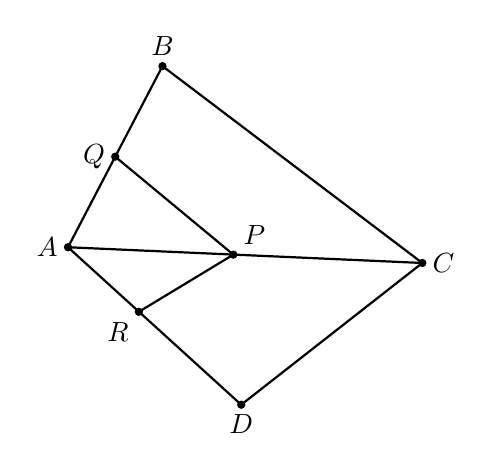
\begin{tikzpicture}[scale=1, thick]
	% Define coordinates for the vertices of quadrilateral ABCD and interior point P
	\coordinate (A) at (1, 2.5);
	\coordinate (B) at (2.2, 4.8);
	\coordinate (C) at (5.5, 2.3);
	\coordinate (D) at (3.2, 0.5);
	\coordinate (P) at (3.1, 2.406);
	
	% Define points Q on AB and R on AD (perpendicular drops from P)
	\coordinate (Q) at (1.6, 3.65);
	\coordinate (R) at (1.9, 1.68);
	
	% Draw quadrilateral ABCD
	\draw (A) -- (B) -- (C) -- (D) -- cycle;
	
	% Draw lines from interior point P to vertices and sides
	\draw (A) -- (C);
	%	\draw (P) -- (A);
	%	\draw (P) -- (B);
	%	\draw (P) -- (C);
	%	\draw (P) -- (D);
	\draw (P) -- (Q);
	\draw (P) -- (R);
	
	% Fill points
	\fill (A) circle (1.5pt);
	\fill (B) circle (1.5pt);
	\fill (C) circle (1.5pt);
	\fill (D) circle (1.5pt);
	\fill (P) circle (1.5pt);
	\fill (Q) circle (1.5pt);
	\fill (R) circle (1.5pt);
	
	% Node labels
	\node[left] at (A) {$A$};
	\node[above] at (B) {$B$};
	\node[right] at (C) {$C$};
	\node[below] at (D) {$D$};
	\node[above right] at (P) {$P$};
	\node[left] at (Q) {$Q$};
	\node[below left] at (R) {$R$};
	
\end{tikzpicture}